%% Benjamin Williams <bwilliams@lincoln.ac.uk>
%% Get in touch if you have any questions or problems!
%% University of Lincoln Computer Science Thesis Template

%% @version     1.0.4
%% @lastchanged 12th June 2020

%% Modified by Mark Doughty
%% University of Lincoln Computer Science Project Report Template
%% @lastchanged 02/03/2022

% The document class -- remove [harvard] if you want
% numeric-style referencing.
\documentclass[harvard]{lincolncsthesis}

% Custom packages that you need to include
% Packages you intend to use
% ..

% For example, if you want to render 
% the document in a different font you can
% use something like: 

% \usepackage{gentium}

\usepackage{url}

% Your thesis details -- edit the file at the path below
% so it shows your name, title, etc. 
% Put the correct details in here
\author{Your Name}
\studentnumber{ABC12345678}
\email{astudent@lincoln.ac.uk}
\thesisDegree{BSc(Hons) Computer Science}
\thesisSubmissionDate{April 2022}

% If your thesis title spans over three lines, prepend the command with \Large!
\title{\bfseries Your Project Title}

% Supervisor details
\thesisSupervisor{Dr. Your Supervisor}

\thesisLogoPath{figures/logo.pdf}  

% Set up the bib files which are gonna be used
% throughout this document
% Add in the .bib files you wish to add 
% into your document here. If you want to
% include others, just copy this line and
% change the path!

\addbibresource{bib/references.bib}


% This thesis template also supports rendering
% a ludography. To cite games, make sure your reference
% in your bib file has keywords={game} in the bibtex item.
%
% See the bib file below for an example.

\addbibresource{bib/ludography.bib}



\begin{document}

% start of document
% --------------------------

% Make the title. You can pass an option to this
% to render the title differently, like so:
%\maketitle[logo-first]
\maketitle

% And so begins the thesis! First include pages
% before the acknowledgements
%% The blank page environment allows you to insert
% pages into your thesis for specific things

\begin{blankpage}
    \chapterTitle{A blank page}
	Here is an optional page environment you could use for things like:
	\begin{itemize}
		\item Your own custom preamble chapters (use \texttt{\textbackslash chapterTitle} for titles!)
		\item \emph{``This work is dedicated to...''}
		\item A copyright notice
		\item Additional notes
		\item Quotes
		\item List of publications
		\item An actual blank page
	\end{itemize}
	You can pass an optional parameter to this environment with the value \texttt{c} to centre this text vertically on the page.
\end{blankpage}

% Acknowledgements
\begin{acknowledgements}
Firstly, I want to thank somebody, and somebody else. Here is another thing.
\end{acknowledgements}
\showthe\font

% The abstract of the thesis
\begin{abstract}
Here is the abstract for this project report.
\end{abstract}

% Print out the table of tables and table of figures and
% tell the template we're about to start the body of the
% thesis.
\thesisTables
\thesisBodyStart


% start of report body
% ---------------------------

% Introduction
\chapter{Introduction}
This document is a project report template for the School of Computer Science, University of Lincoln. It should give you some direction and instruction for formatting and presenting your project report. If you have any suggestions or issues, please contact the creator of the template on which this is based, \texttt{bwilliams@lincoln.ac.uk} or \texttt{jamesbrown@lincoln.ac.uk}. Currently, this template is designed for undergraduate project reports. However, the template can be modified fairly easily to conform to, for example, an MComp project report.

This document has been generated using \LaTeX, which is a widely used typesetting system in computer science, engineering, and other STEM disciplines. The following subsections of this chapter demonstrate some basic \LaTeX commands. If you would prefer to use the supplied LNCS Word template, then you should aim to replicate the formatting shown here.

\section{Formatting mathematics}
Here are two equations:

\begin{align}
a &= b + 1 \\
\frac{\hbar^2}{2m}\nabla^2\Psi + V(\mathbf{r})\Psi
&= -i\hbar \frac{\partial\Psi}{\partial t}    
\end{align}


And here is some text with some nice inline maths, $(x, y)$ wow $\gamma$ so cool $\rho$.

\section{Figures and Tables}

Here is a sentence, and you can see a nice picture in Figure \ref{fig:brayford}.

\begin{figure}[h]
    \centering
    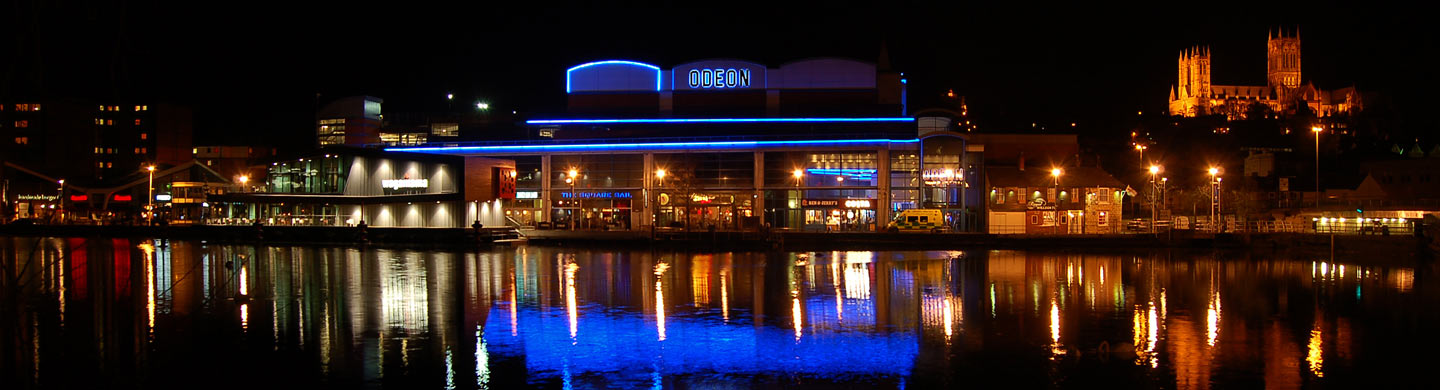
\includegraphics[width=\textwidth]{figures/brayford.jpg}
    \caption{A picture of the Brayford from Google Images.}
    \label{fig:brayford}
\end{figure}

Also, a table can be found in Table \ref{tbl:example-table}. You should use a \LaTeX~table generator like \url{https://www.tablesgenerator.com/} if you want to make your life easier.

\begin{table}[h]
    \caption{Here is a table. The caption goes above like this.}
    \centering
    \begin{tabular}{l|l|c}
        First name & Last name & Age \\
        \hline\hline
        Bob & Bobbington & 24 \\
        Benth & Wavies & 49 \\
        Joe & Bloggs & 37 \\
        Billy & Bob & 10 \\

    \end{tabular}
    \label{tbl:example-table}
\end{table}

\section{Referencing}
The included \texttt{[harvard]} in the document class command means that referencing will follow a Harvard style. You will be able to cite things inline with parentheses. You can do this by using \texttt{\textbackslash citep\{citekey\}}. It will print out something like this \citep{aad2012observation}. Or alternatively, you can use \texttt{\textbackslash cite\{citekey\}} to cite things like this \cite{chatrchyan2012observation}.

It is worth noting that the standard for referencing is Harvard, so you will not need to change this option. However, please double and triple check this to make sure you are using the correct referencing style. Also, ask your supervisor to make sure. This template uses Bib\LaTeX~for referencing, with a Biber backend. This is primarily due to the extensive features Bib\LaTeX~provides, along with the option of glossaries. If you want to customise the referencing style, you can either modify the template slightly to use different options, or use \texttt{\textbackslash usepackage} again to reimport it. There's probably some commands to change its options after its been imported too.

\subsection{Ludography}
This report template also contains an optional ludography. For Games Computing students to use this, just put references into your bib file as usual with the game's details. Then, make sure \texttt{keywords} is set to \texttt{\{game\}}. This is what is used to determine which references are games, and which are actual papers. For a more elaborate example, see \texttt{bib/ludography.bib}.

Also, make sure that the \texttt{title} key is actually the author of the game, and the \texttt{author} is the title of the game. The reason this is swapped around is because Bib\LaTeX~likes to print references out with the author first.

Then, just add \texttt{\textbackslash printLudography} with an optional title argument to print out all citations like \texttt{\textbackslash printLudography} or \texttt{\textbackslash printLudography[Games]}.

You can also use the \texttt{ludography} environment if you wish to print out some text before the list of games is printed. An example of this can be seen in \texttt{main.tex}.

To cite games, you can \texttt{\textbackslash cite} it like any other reference. However, if you want it to display the title instead of the standard referencing style, you can use \texttt{\textbackslash citeGame} instead.

 
% Literature review
\chapter{Literature Review}
The literature review is an essential requirement of any academic project. A comprehensive review of the literature will provide background to the project, and should be used to inform a set of requirements that your solution must meet. It also establishes that what you have done is the result of academic study, rather than an unfounded whim. This section can use the literature review submitted as part of the Interim Report. You should use the feedback from your supervisor to improve upon the final version. 

It may be helpful to break up this chapter into sections, with each focused on a different topic or aspect of the project.

\section{Aims \& Objectives}
Having situated your project within a body of relevant literature, you should now be in a position to state your aims and objectives. These should be broadly similar to those given in your proposal. Most projects will have one aim that is a broad statement of what the project will achieve. The objectives should be statements of how that aim will be achieved. Objectives should be Specific, Measurable, Assignable, Realistic and Time-related (SMART).

% Requirements analysis
\chapter{Requirements Analysis}
Drawing upon the research you've conducted, the goal of this chapter is to formalise a set of requirements that project must fulfil in order to meet your objectives. This chapter can be relatively short, and reference the aim(s) \& objectives given at the end of the previous chapter. 

For software-oriented projects, consider key stakeholders (end-users, business owners) when analysing the requirements of your software. This may be through primary research (i.e., interviews with potential end-users or clients) or secondary research (e.g., literature review, survey of existing products). For research-oriented projects, use your literature survey to highlight current gaps in knowledge that you hope to address. Consider what your artefact must do in order to obtain meaningful results.

% Design & Methodology
\chapter{Design \& Methodology}
This section of the dissertation may vary significantly in both structure and content, depending on the type of project you are undertaking. However, it is expected that all projects have the following sections:

\begin{itemize}
    \item Project management
    \item Risk analysis
\end{itemize}

The precise structure should be discussed with your supervisor, but some suggestions for additional sections are given below. The key thing to note here is that irrespective of the project type, you should \emph{justify} the choices you've made, rather than simply choosing based on expediency or familiarity.

\section{Software development projects}
\label{sd-projects}

If the primary deliverable of your project is a software product, then you should consider subsections detailing your approaches to the following:

\begin{itemize}
    \item Software development methodology (e.g., waterfall, scrum)
    \item Toolsets and machine environments (i.e., the software and hardware used)
    \item Design (e.g., UML diagrams, database schema, prototypes)
    \item Testing (i.e., the types of testing used)
\end{itemize}

This list is not exhaustive. For example, a games design project may include a game design document. However, it must be noted that if your project contains significant software development work, then most if not all of these sections should be present.

\section{Research \emph{not} involving human participants}

For some projects, the main deliverables may come in the form of experimental results. For example, a project comparing several different algorithms may require little in the way of code, but require considerable experimentation and data analysis. As such, all methodological choices made should be documented here. Examples include:

\begin{itemize}
    \item Dataset acquisition and annotation
    \item Algorithm/model design and selection
    \item Parameter tuning
    \item Performance metrics
\end{itemize}

Again, this list is not exhaustive, and you should still include relevant sections pertaining to the software artefact listed in Section \ref{sd-projects}.

\section{Research involving human participants}

For projects involving human participants, you will need to consider a hypothesis or research question that your project will answer. In addition to the sections outlined in Section \ref{sd-projects}, you may also need to provide details of:

\begin{itemize}
    \item Participant recruitment
    \item Evidence that ethical procedures have been followed
    \item Study design (including hypotheses/research question as appropriate)
    \item Statistical analysis (i.e., how you'll analyse the raw data)
\end{itemize}

If your study involves data collection by means of questionnaires, you may also wish to specify the questions here (or refer to them in an appendix).

% Implementation
\chapter{Implementation}
This section should demonstrate your solution from a technical perspective, showing the different components of your software. You may wish to include code snippets and screenshots as figures to provide detail where necessary.

% Results & Discussion
\chapter{Results \& Discussion}
This section should present the findings of your work, and discuss them in the context of your original aims \& objectives as well as your requirements specification. For software-oriented projects, how well does it meet your original requirements? Provide data where possible, e.g., results of user testing, performance measures, etc. For research-oriented projects, you should present the data in an appropriate format (tables, charts, visualisations) and discuss what the data shows.

% Conclusion
\chapter{Conclusion}
This is another relatively short chapter that is an opportunity to reflect on the project as a whole. Discuss the limitations and successes of the project, highlighting opportunities for future work. 



% end of thesis body
% --------------------------

% Print out the references
\printReferences

% Print out the ludography (optional)
\printLudography

% If you want to put some text before the list of games,
% then you can use the following code:
%\begin{ludography}[Ludography / Optional Title]
    %Here are some games.
%\end{ludography}


\end{document}
